%%%%%%%%%%%%%%%%%%%%%%%%%%%%%%%%%%%%%%%%%%%%%%%%%%%%%%%%%%%%%%%%%%%%%%%%%%%%%%%%
%2345678901234567890123456789012345678901234567890123456789012345678901234567890
%        1         2         3         4         5         6         7         8
% THESIS CHAPTER

\chapter{The algorithms}
\label{chap:algorithms}
\ifpdf
    \graphicspath{{Algorithms/Figures/PNG/}{EvaluationTask/Figures/PDF/}{Algorithms/Figures/}}
\else
    \graphicspath{{Algorithms/Figures/EPS/}{EvaluationTask/Figures/}}
\fi


% short summary of the chapter
The main algorithms analysed in the project are attempted to be as different as
possible from each other. This allows covering as many audio features and
similarity measuring techniques as possible. My motivations of the choice of
algorithms were influenced by the study on MIREX submissions, as well as the
overall scope of features they encompass. 

Julien Osmalsky coins the term \textit{rejector} to define a pairwise comparison
function that given two audio tracks it returns a score ranking of similarity
between both tracks \cite{osmalsky2015combining}. This term was adopted by the
project to refer to each of the algorithms examined. The relation between an
algorithm paper and its rejector term is outlined in section \ref{sec:algolist}.

The final selection includes 5 individual algorithms and an algorithm
aggregating results from 4 of them. Each of the algorithms is examined
individually, with the results from some of them combined through the rank
aggregation algorithm.


\section{Algorithms list}
\label{sec:algolist}
The analysis if performed on the following algorithm:
\begin{itemize}
    \item \textbf{Weak rejector} - Osmalskyj, Julien, Marc Van Droogenbroeck,
    and Jean-Jacques Embrechts. \textit{Enhancing cover song identification with
    hierarchical rank aggregation} \cite{osmalsky2016enhancing}
    \item \textbf{Cross-correlation rejector} - Ellis, Daniel PW, Courtenay V.
    Cotton, and Michael I. Mandel. \textit{Cross-correlation of beat-synchronous
    representations for music similarity} \cite{ellis2008cross}
    \item \textbf{Quantisation rejector} - Osmalskyj, Julien, et al.
    \textit{Combining features for cover song identification} \cite{osmalsky2015combining}
    \item \textbf{Timbre rejector} - Tralie, Christopher J., and Paul Bendich.
    \textit{Cover song identification with timbral shape sequences} \cite{tralie2015cover}
    \item \textbf{Aggregated rank rejector} - Osmalskyj, Julien, Marc Van
    Droogenbroeck, and Jean-Jacques Embrechts. \textit{Enhancing cover song
    identification with hierarchical rank aggregation}
    \cite{osmalsky2016enhancing} 
    \item \textbf{Fingerprint rejector} - Rafii, Zafar, Bob Coover, and Jinyu
    Han. \textit{An audio fingerprinting system for live version identification
    using image processing techniques} \cite{rafii2014audio}
\end{itemize}

\begin{figure}[H]
    \centering
    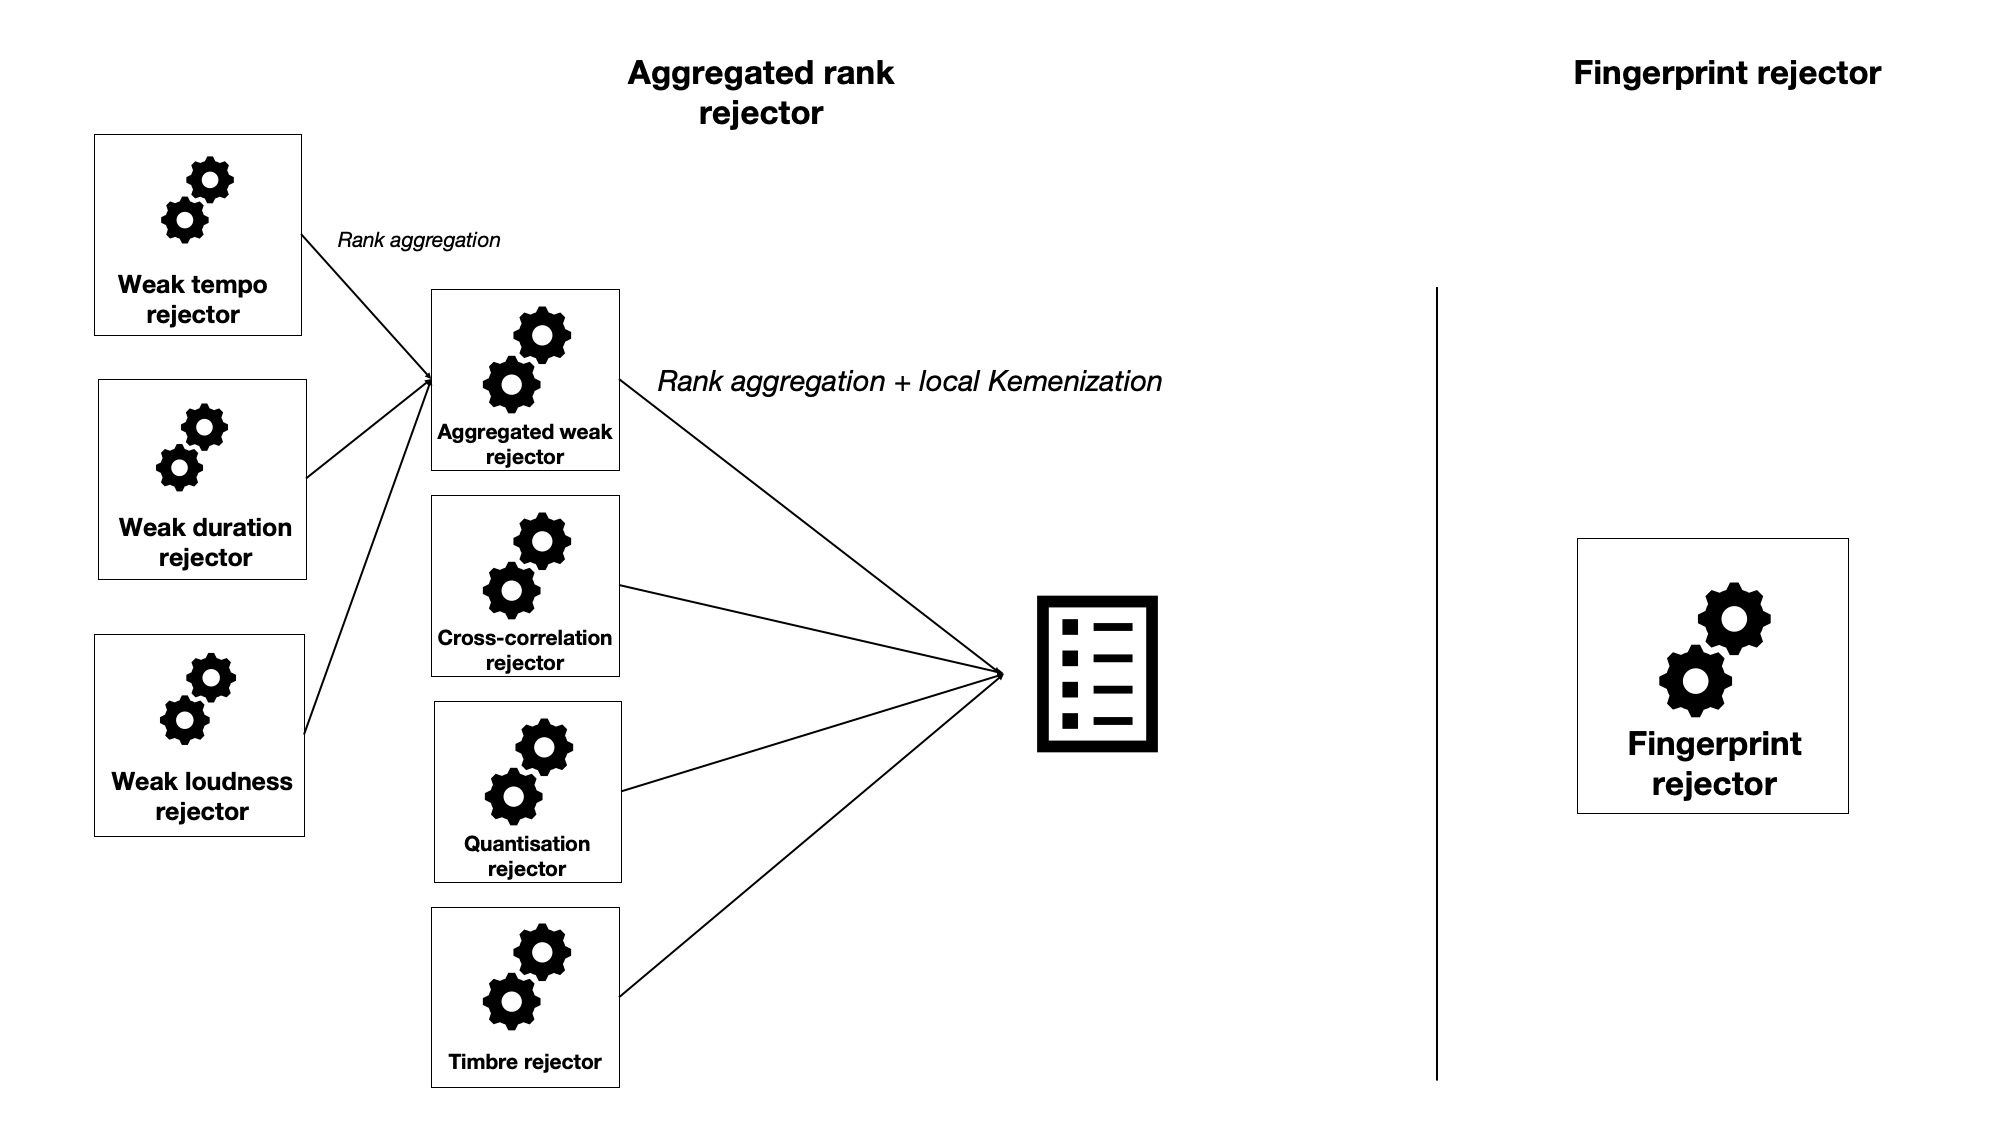
\includegraphics[width=\textwidth]{Algorithms/algorithm_diagram_3.jpg}
    \captionof{figure}[Algorithms diagram]{Diagram of chosen algorithms and the relationships between them. The aggregated rank rejector combines the results of 3 types of weak rejectors, as well as the quantisation, cross-correlation and timbre rejectors.}
    \label{fig:algorithms}
\end{figure}

\section{Weak rejector} 
\label{sec:osmalskyj}

The weak rejector takes its name from the fact that it uses global single-valued
features of sound to calculate a similarity score. Weak features include tempo,
duration, loudness, average number of beats, etc. Those audio properties are
considered 'weak' since by themselves they cannot uniquely describe a song - the
majority of pop tracks from a certain era are composed with the same tempo, for
example \cite{slowpop}. As a consequence the results from weak rejectors are
inherently insignificant are usually not considered individually, but as
part of an aggregation with other results.

Each weak rejector takes a single audio feature as song representation. The
algorithm extracts the feature from each song in a dataset and from them it
creates a training set by combining each pair of songs in different ways. For
songs $A$ and $B$ with weak feature values of $f1$ and $f2$ respectively the
minimum ($min(f1, f2)$), maximum ($max(f1, f2)$), sum ($f1 + f2$), quotient
($\frac{f1}{f2}$) and absolute value of quotient of the difference divided by
the sum ($abs(\frac{f1 - f2}{f1 + f2})$) are taken. The generated data is used
as attributes to train an ExtraTrees classifier model. Extra randomised trees or
ExtraTrees classification is a form of random forest classification. In
contrast to the regular random forest implementation, ExtraTrees uses the whole
training data for each decision tree. Rather than calculating an optimal
cut-point, it also uses a random one. The direct benefits of using this
variation of random trees are higher computational efficiency while achieving
similar perfomance on average, in addition to better results on some specific
problems \cite{geurts2006extremely}.

The evaluation datasets used in this project are too small to generate an
ExtraTrees model which performs even adequate classification of songs. To gather
sufficient training data the weak features of 12,104 songs are extracted from
the music streaming service Spotify \cite{spotify}. The tracks are chosen based
on clique groupings from the SecondHandSongs (SHS) \cite{shs} dataset - the
largest dataset of covers songs aimed at academic research. While the full
dataset is difficult to obtain, information about the cliques structure within
it is easy to find. The extracted data is then combined into pairs using the
procedure outlined in the previous paragraph. A binary class is then assigned to
each pair entry depending on whether the pair of songs are covers or not.
Afterwards the training data is further split into a training set of 3773
cliques (8653 songs) and validation set containing 1573 cliques (3451 songs).
The metric used to validate the model performance is the area under the receiver
operating characteristic (ROC) curve - a curve resulting from the plot of the
true positive against the false positive rate of the validation results. ROC
analysis of such form is suitable as a validation metric for the selection of an
optimal model because it is independent of any potential cost function or cost
distribution \cite{wiki:roc}. Because we are solely working with weak feature
information the we can only validate based on correct and incorrect produced results.

After the training phase is complete each of the evaluation datasets is
converted into the training set format and passed to the model for class
prediction. The output result is a probability of every pair of songs being
covers. Grouping the results per song produces a database ordering that is
required by the evaluation task.
\section{Cross-correlation rejector} 
\label{sec:weakfeatures}
The cross-correlation rejector uses chroma features as the main audio feature
describing each song. Being a powerful representation of the distinct 12
semitones part of an octave, they are very similar to the harmonic pitch class
profiles (HPCPs) discussed earlier. 
\section{Quantisation rejector} 
\label{sec:ccs}
\section{Timbre rejector} 
\label{sec:quantisation}
\section{Aggregated rank rejector} 
\label{sec:timbre}
\section{Fingerprint rejector} 
\label{sec:rankaggregation}

